% !TeX root = ../../main.tex
\graphicspath{{Parts/3_Integrations/graphics/}}
\subsection{Overleaf}
The best way to use local \LaTeX{} is \emph{in conjunction with}, and not instead of Overleaf. Overleaf does have its own strengths after all, due to its real time collaboration ability. Overleaf and local versions of \LaTeX{} can be integrated into one seamless experience using Github (although, the owner of the document must have Overleaf premium for this feature). This can be done as follows
\begin{enumerate}
    \item Have your \LaTeX{} project in a Github repository. It is fine if your repo consists of other files such as project code, but keep in mind that Overleaf project sizes are limited to 100MB. If the Github repo for your project is larger than this, then it is probably better to save your writeup as a submodule in the project repository (and use this submodule as the repository for the \LaTeX{} project itself).
    \item Connect your Overleaf account to your Github account through your account settings
    \item Now, when creating a new project, select the option to import from Github
    \begin{figure}[ht!]
        \centering
        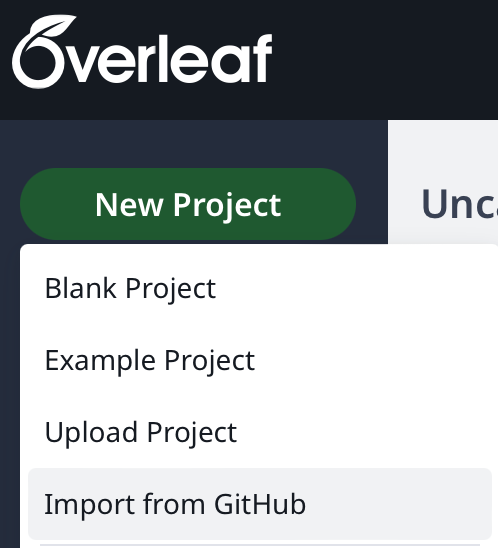
\includegraphics[width = 0.4\textwidth]{new}
        \caption{Importing a project from Github}
    \end{figure}
    This will give you a drop down box of your Github repos. Select the one you wish to import into Overleaf. Note that this will import EVERY file in the repository into overleaf, so if you have your \LaTeX{} stuff saved into a submodule, import that. Once you do this, Overleaf should automatically identify your main tex file, although if it does that improperly you can always set it in the project menu.

    \item 
    Now that you've connected Overleaf and Github, you can push and pull commits between them using Overleaf as a remote repository through the project menu bar. You will see this screen
    \newpage
    \begin{figure}[ht!]
        \centering
        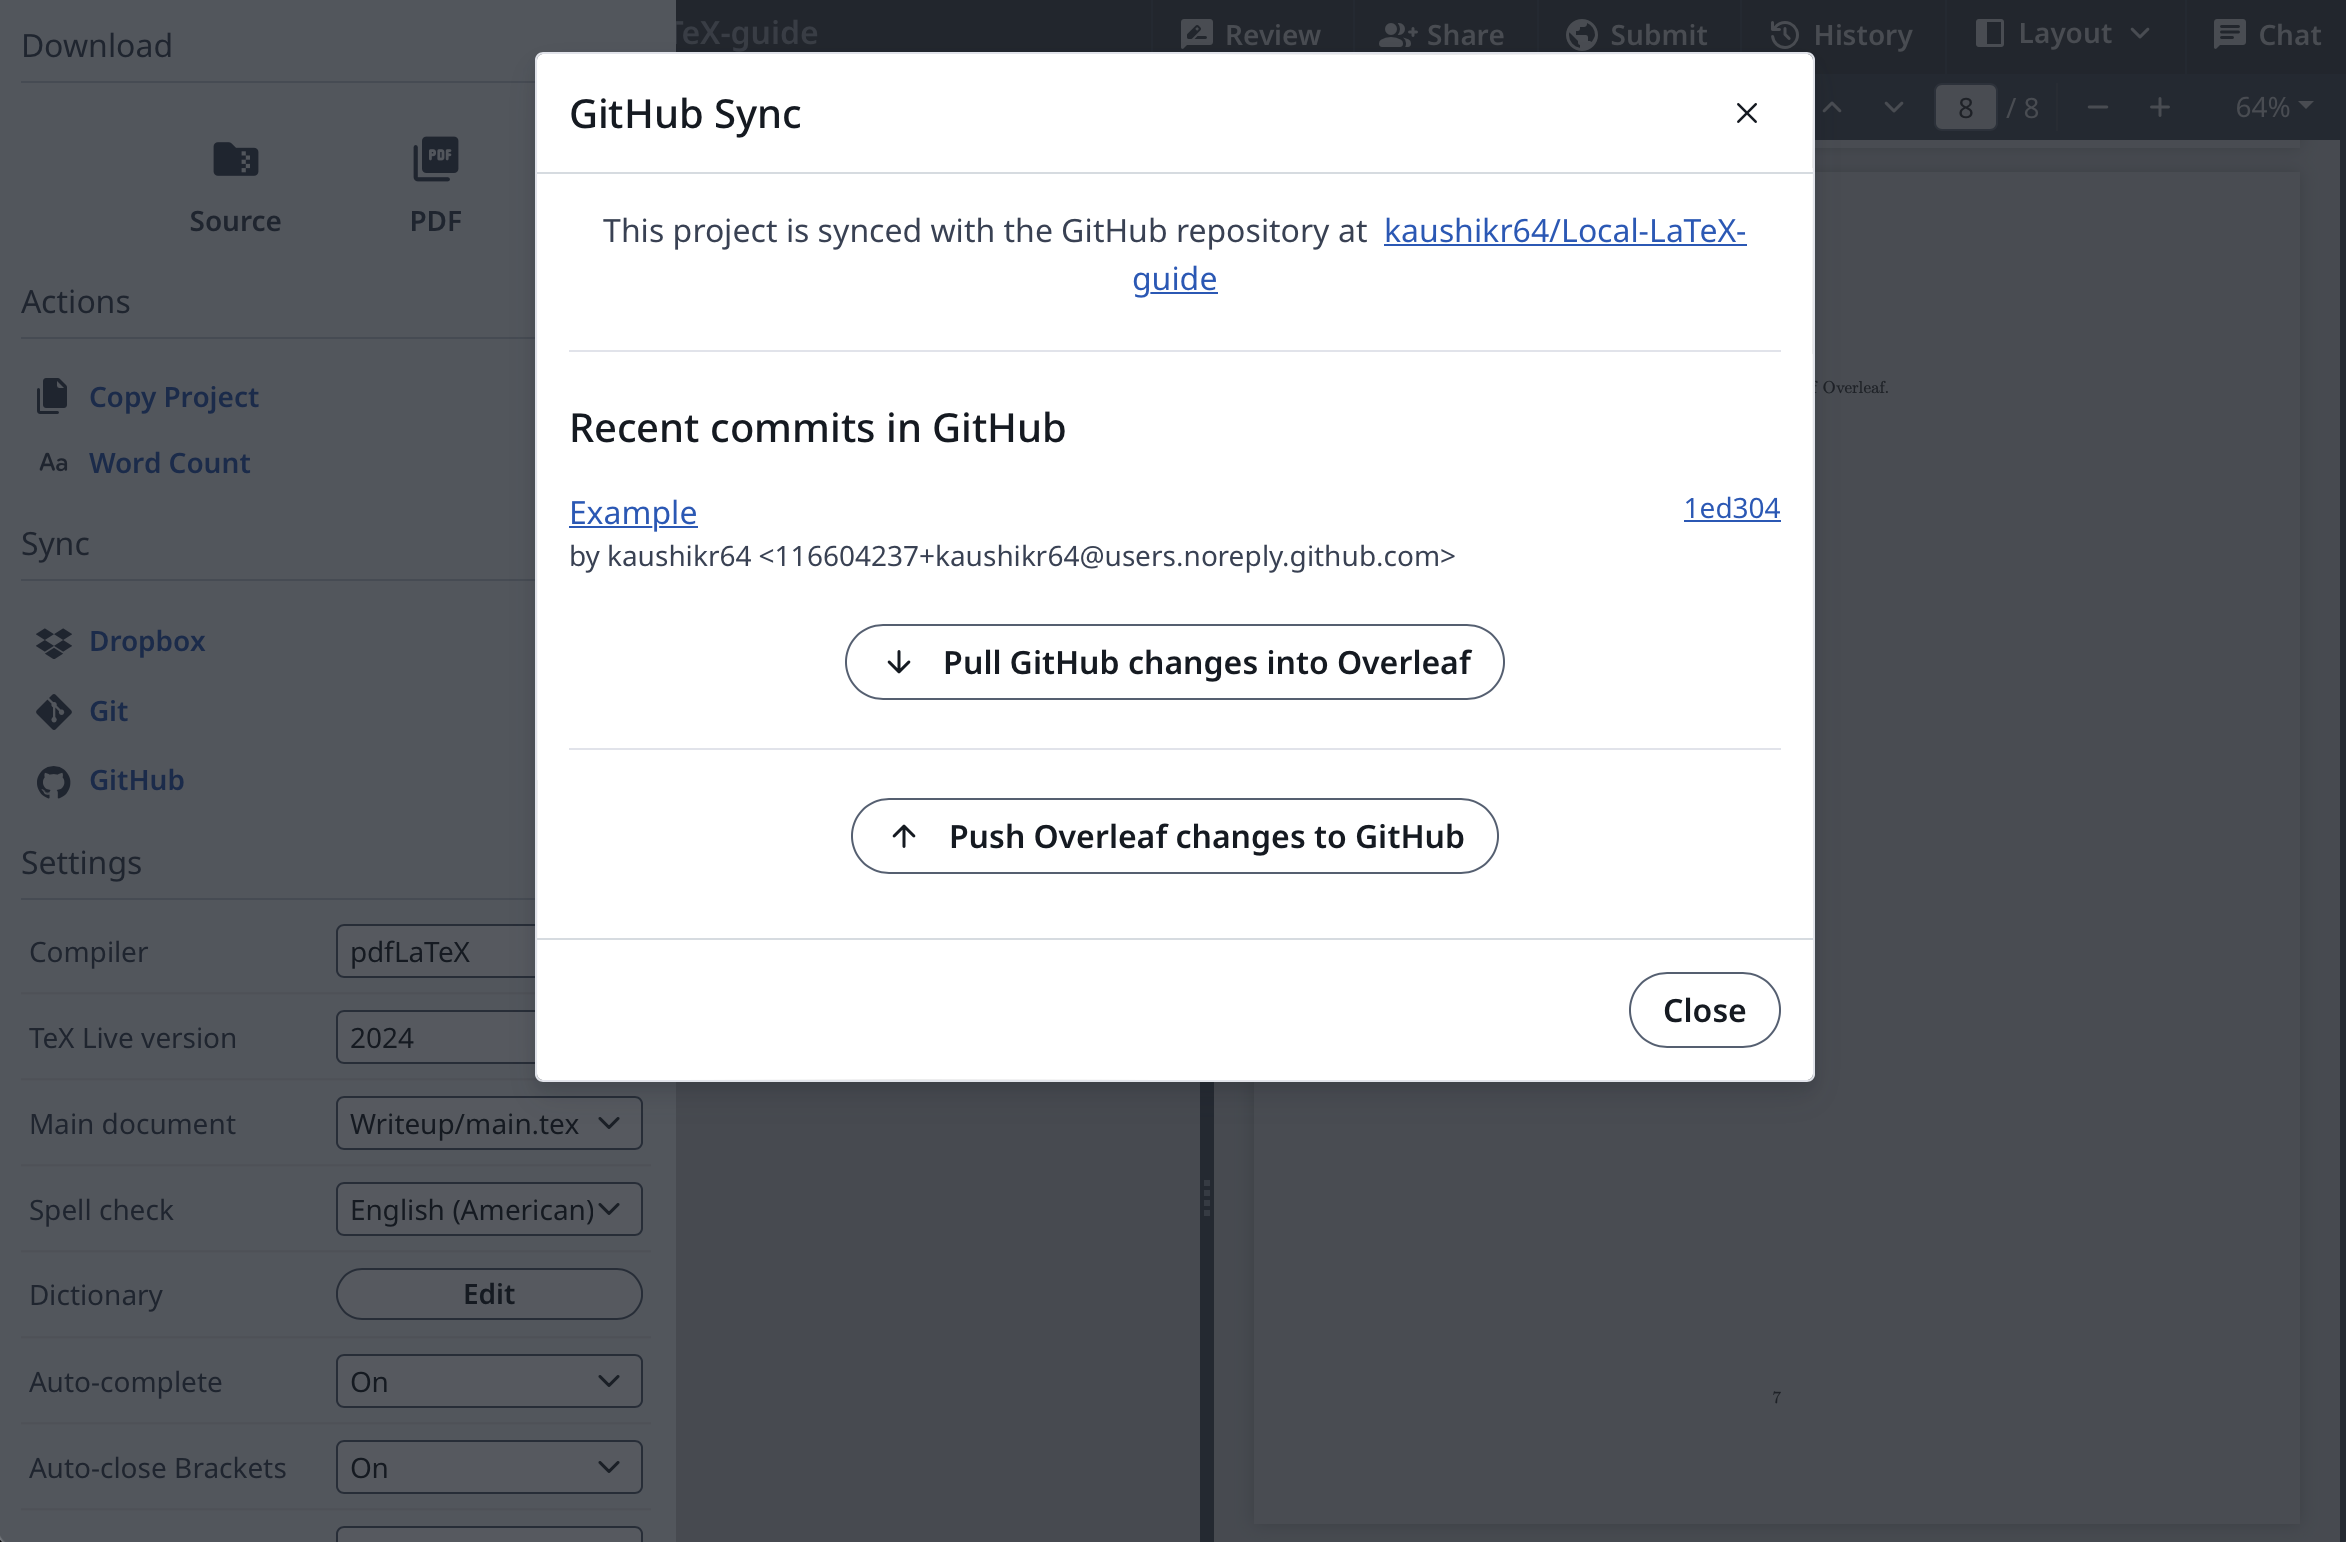
\includegraphics[width = 0.8\textwidth]{sync}
        \caption{Github Sync screen, you can get here by pressing Github under the sync options to the left}
    \end{figure}
    You can now pull/push commits as necessary. Any user given edit access to the overleaf document can pull and push changes to the Github repo even if it is private, so this allows for easy collaboration with others

    \item 
    Suppose you already have an Overleaf document, and wish to update it locally, this can also be done by creating a Github repo through Overleaf itself for the project. Simply navigate to the project menu once more and click the Github option under the sync options. This brings up the following page
    \begin{figure}[ht!]
        \centering
        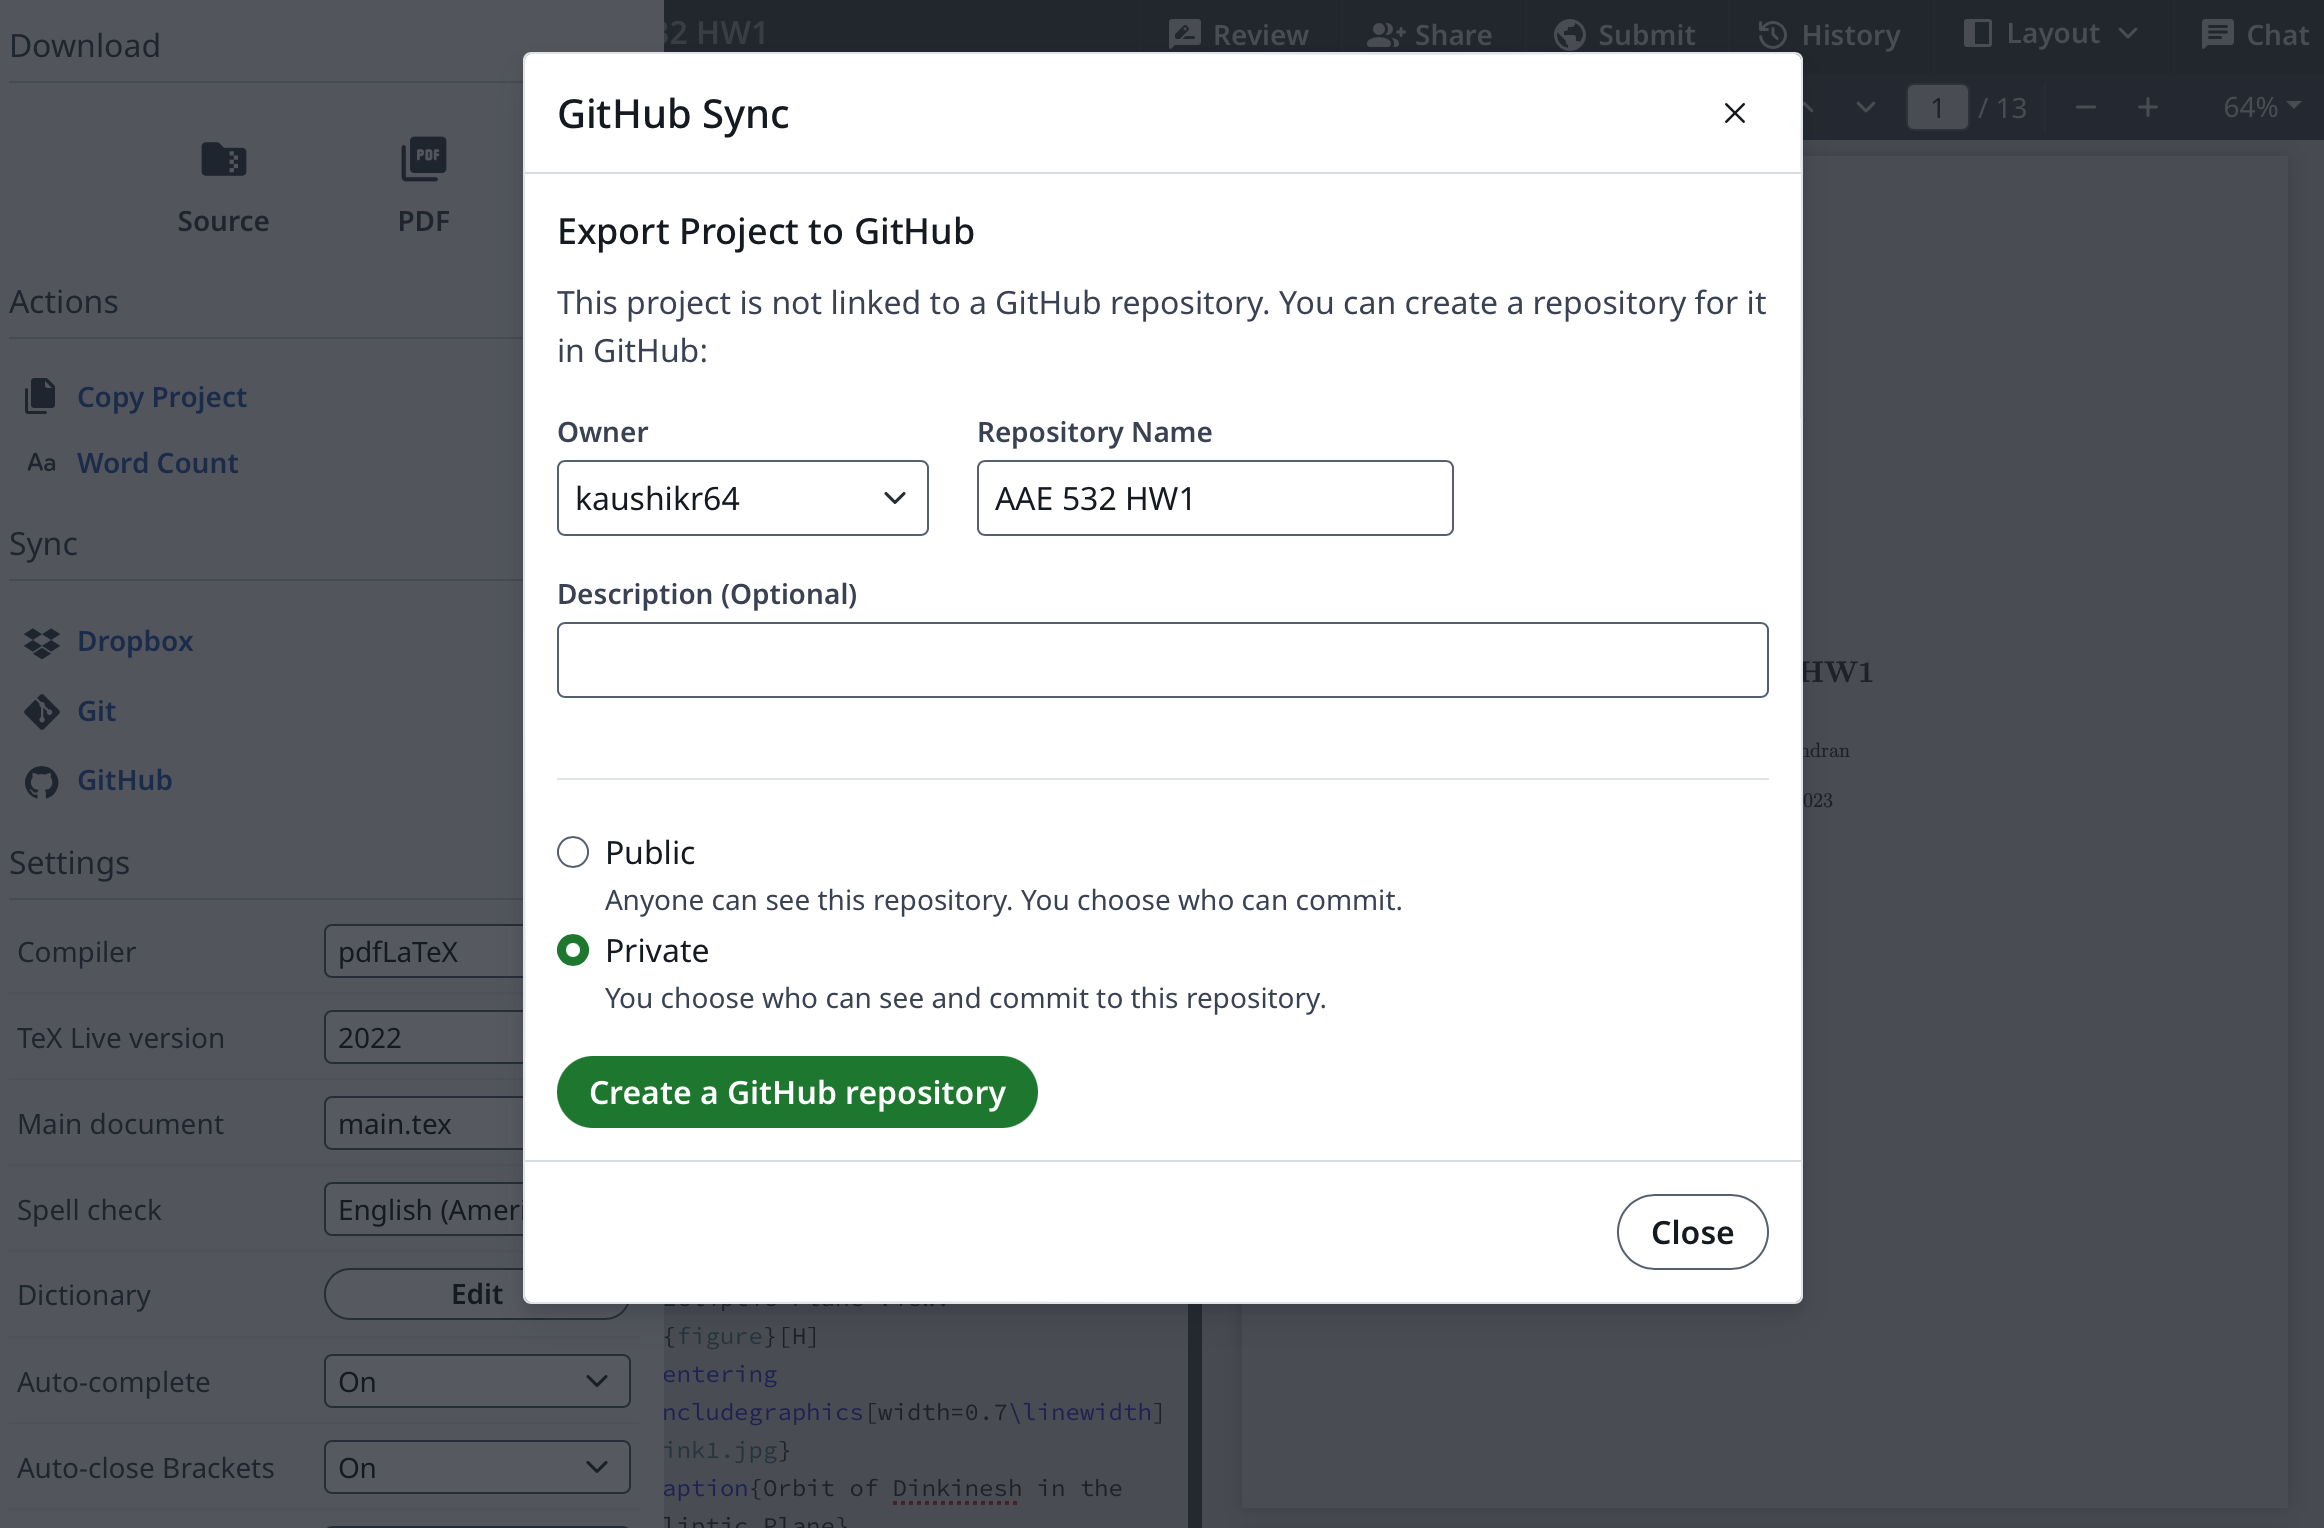
\includegraphics[width = 0.7\textwidth]{reoi}
        \caption{Create a Github repo from an existing Overleaf project}
    \end{figure}
    
    After using this menu to create a Github repo, you can clone it to your local machine and start using your local \LaTeX{} setup. From here syncing Github and Overleaf works the same way as before.
\end{enumerate}

